\documentclass[a4paper]{book}
\usepackage{makeidx}
\usepackage{graphicx}
\usepackage{multicol}
\usepackage{float}
\usepackage{listings}
\usepackage{color}
\usepackage{ifthen}
\usepackage[table]{xcolor}
\usepackage{textcomp}
\usepackage{alltt}
\usepackage{ifpdf}
\ifpdf
\usepackage[pdftex,
            pagebackref=true,
            colorlinks=true,
            linkcolor=blue,
            unicode
           ]{hyperref}
\else
\usepackage[ps2pdf,
            pagebackref=true,
            colorlinks=true,
            linkcolor=blue,
            unicode
           ]{hyperref}
\usepackage{pspicture}
\fi
\usepackage[utf8]{inputenc}
\usepackage{mathptmx}
\usepackage[scaled=.90]{helvet}
\usepackage{courier}
\usepackage{doxygen}
\lstset{language=C++,inputencoding=utf8,basicstyle=\footnotesize,breaklines=true,breakatwhitespace=true,tabsize=8,numbers=left }
\makeindex
\setcounter{tocdepth}{3}
\renewcommand{\footrulewidth}{0.4pt}
\begin{document}
\hypersetup{pageanchor=false}
\begin{titlepage}
\vspace*{7cm}
\begin{center}
{\Large PG\_\-Btree \\[1ex]\large 0.1 }\\
\vspace*{1cm}
{\large Generated by Doxygen 1.7.3}\\
\vspace*{0.5cm}
{\small Wed Apr 4 2012 17:58:22}\\
\end{center}
\end{titlepage}
\clearemptydoublepage
\pagenumbering{roman}
\tableofcontents
\clearemptydoublepage
\pagenumbering{arabic}
\hypersetup{pageanchor=true}
\chapter{Class Index}
\section{Class Hierarchy}
This inheritance list is sorted roughly, but not completely, alphabetically:\begin{DoxyCompactList}
\item \contentsline{section}{BTree$<$ T, Cmp $>$}{\pageref{classBTree}}{}
\item \contentsline{section}{BTree$<$ T, Cmp $>$::generic\_\-iterator}{\pageref{classBTree_1_1generic__iterator}}{}
\begin{DoxyCompactList}
\item \contentsline{section}{BTree$<$ T, Cmp $>$::iterator}{\pageref{classBTree_1_1iterator}}{}
\item \contentsline{section}{BTree$<$ T, Cmp $>$::reverse\_\-iterator}{\pageref{classBTree_1_1reverse__iterator}}{}
\end{DoxyCompactList}
\item \contentsline{section}{Node$<$ T, Cmp $>$}{\pageref{classNode}}{}
\end{DoxyCompactList}

\chapter{Class Index}
\section{Class List}
Here are the classes, structs, unions and interfaces with brief descriptions:\begin{DoxyCompactList}
\item\contentsline{section}{\hyperlink{classBTree}{BTree$<$ T, Cmp $>$} (Conainter class. Store Nodes in a Tree )}{\pageref{classBTree}}{}
\item\contentsline{section}{\hyperlink{classBTree_1_1generic__iterator}{BTree$<$ T, Cmp $>$::generic\_\-iterator} }{\pageref{classBTree_1_1generic__iterator}}{}
\item\contentsline{section}{\hyperlink{classBTree_1_1iterator}{BTree$<$ T, Cmp $>$::iterator} }{\pageref{classBTree_1_1iterator}}{}
\item\contentsline{section}{\hyperlink{classNode}{Node$<$ T, Cmp $>$} (\hyperlink{classBTree}{BTree} \hyperlink{classNode}{Node}. Contains Elements/Keys )}{\pageref{classNode}}{}
\item\contentsline{section}{\hyperlink{classBTree_1_1reverse__iterator}{BTree$<$ T, Cmp $>$::reverse\_\-iterator} }{\pageref{classBTree_1_1reverse__iterator}}{}
\end{DoxyCompactList}

\chapter{Class Documentation}
\hypertarget{classBTree}{
\section{BTree$<$ T, Cmp $>$ Class Template Reference}
\label{classBTree}\index{BTree@{BTree}}
}


Conainter class. Store Nodes in a Tree.  


\subsection*{Classes}
\begin{DoxyCompactItemize}
\item 
class \hyperlink{classBTree_1_1generic__iterator}{generic\_\-iterator}
\item 
class \hyperlink{classBTree_1_1iterator}{iterator}
\item 
class \hyperlink{classBTree_1_1reverse__iterator}{reverse\_\-iterator}
\end{DoxyCompactItemize}
\subsection*{Public Member Functions}
\begin{DoxyCompactItemize}
\item 
\hyperlink{classBTree_a83e51e388096d95b5521e8058bad44ed}{BTree} (int lower=2, int upper=-\/1)
\begin{DoxyCompactList}\small\item\em Make an new empty Tree. \item\end{DoxyCompactList}\item 
\hypertarget{classBTree_a2de4cbb350239a4af75aa7013a6a4d81}{
\hyperlink{classBTree_a2de4cbb350239a4af75aa7013a6a4d81}{$\sim$BTree} ()}
\label{classBTree_a2de4cbb350239a4af75aa7013a6a4d81}

\begin{DoxyCompactList}\small\item\em Destroy the entire Tree, and its Nodes. \item\end{DoxyCompactList}\item 
void \hyperlink{classBTree_aad8382a0461d68609f4a7ac6ff129b13}{insertElement} (const T \&element)
\begin{DoxyCompactList}\small\item\em Insert and sort a new element in the Tree. \item\end{DoxyCompactList}\item 
int \hyperlink{classBTree_a4a16f1104c087b066c112fb3d9bd9d67}{removeElement} (T element)
\begin{DoxyCompactList}\small\item\em Find and remove an element from the Tree. \item\end{DoxyCompactList}\item 
\hyperlink{classNode}{Node}$<$ T, Cmp $>$ $\ast$ \hyperlink{classBTree_af33992c6615d26590eec8c9c4f3a84de}{findElementNode} (const T \&element)
\begin{DoxyCompactList}\small\item\em Find an element in the Tree. \item\end{DoxyCompactList}\item 
\hyperlink{classNode}{Node}$<$ T, Cmp $>$ $\ast$ \hyperlink{classBTree_a3d649eb521392e1a6172e08ddd965a1b}{getRootNode} ()
\begin{DoxyCompactList}\small\item\em Access to root \hyperlink{classNode}{Node}. \item\end{DoxyCompactList}\item 
\hypertarget{classBTree_afd84bd36b0ac7b91c578b08cb5bf364c}{
void {\bfseries draw} (std::ostream \&flux) const }
\label{classBTree_afd84bd36b0ac7b91c578b08cb5bf364c}

\item 
int \hyperlink{classBTree_a3bb7a75716764713beb317b80ff32238}{size} ()
\begin{DoxyCompactList}\small\item\em Get number of elements in the Tree. \item\end{DoxyCompactList}\item 
\hyperlink{classBTree_1_1iterator}{iterator} \hyperlink{classBTree_aeb805dd429fe16186845e66e67a7e498}{begin} ()
\begin{DoxyCompactList}\small\item\em Create a new iterator refering to the first element. \item\end{DoxyCompactList}\item 
\hyperlink{classBTree_1_1reverse__iterator}{reverse\_\-iterator} \hyperlink{classBTree_a0fd7a5d6f77b6d55d1a6f12a6015159b}{rbegin} ()
\begin{DoxyCompactList}\small\item\em Create a new \hyperlink{classBTree_1_1reverse__iterator}{reverse\_\-iterator} refering to the last element. \item\end{DoxyCompactList}\item 
\hyperlink{classBTree_1_1iterator}{iterator} \hyperlink{classBTree_a84ac54a58e8fa886e6d3a61cef1ab8ad}{end} ()
\begin{DoxyCompactList}\small\item\em Create a new iterator refering to end. \item\end{DoxyCompactList}\item 
\hyperlink{classBTree_1_1reverse__iterator}{reverse\_\-iterator} \hyperlink{classBTree_ad2d647f5b6335d9ea5b9d34f5cb707d4}{rend} ()
\begin{DoxyCompactList}\small\item\em Create a new \hyperlink{classBTree_1_1reverse__iterator}{reverse\_\-iterator} refering to end. \item\end{DoxyCompactList}\item 
\hypertarget{classBTree_a74c65eb308a4351ada51582cec3ae7ea}{
\hyperlink{classBTree_1_1iterator}{iterator} {\bfseries root} ()}
\label{classBTree_a74c65eb308a4351ada51582cec3ae7ea}

\end{DoxyCompactItemize}
\subsection*{Public Attributes}
\begin{DoxyCompactItemize}
\item 
\hypertarget{classBTree_a01ae7e4c943cf39a84c01e738cf54e30}{
int {\bfseries \_\-dbg}}
\label{classBTree_a01ae7e4c943cf39a84c01e738cf54e30}

\end{DoxyCompactItemize}
\subsection*{Protected Member Functions}
\begin{DoxyCompactItemize}
\item 
\hypertarget{classBTree_abfec9fc638844e35afc65644ac18efc4}{
void \hyperlink{classBTree_abfec9fc638844e35afc65644ac18efc4}{addToNode} (\hyperlink{classNode}{Node}$<$ T, Cmp $>$ $\ast$node, const T \&element)}
\label{classBTree_abfec9fc638844e35afc65644ac18efc4}

\begin{DoxyCompactList}\small\item\em Safe element insertion in a \hyperlink{classNode}{Node}. Call automatically splitNode when necessary. \item\end{DoxyCompactList}\item 
\hypertarget{classBTree_a987f244ae4a949d2a8bfc37fbb3f6bd1}{
int \hyperlink{classBTree_a987f244ae4a949d2a8bfc37fbb3f6bd1}{removeFromNode} (\hyperlink{classNode}{Node}$<$ T, Cmp $>$ $\ast$node, const T \&element)}
\label{classBTree_a987f244ae4a949d2a8bfc37fbb3f6bd1}

\begin{DoxyCompactList}\small\item\em Safe element deletion in a \hyperlink{classNode}{Node}. Call automatically balanceNode when necessary. \item\end{DoxyCompactList}\item 
void \hyperlink{classBTree_a17124d656659761322bf2a5d175225e0}{mergeNodes} (\hyperlink{classNode}{Node}$<$ T, Cmp $>$ $\ast$targetNode, \hyperlink{classNode}{Node}$<$ T, Cmp $>$ $\ast$sourceNode)
\begin{DoxyCompactList}\small\item\em Merge a source \hyperlink{classNode}{Node} in a target \hyperlink{classNode}{Node}. SubNodes are also transferred. \item\end{DoxyCompactList}\item 
void \hyperlink{classBTree_aa4d84b1d728a3d4b170821c14cb82d0d}{splitNode} (\hyperlink{classNode}{Node}$<$ T, Cmp $>$ $\ast$node)
\begin{DoxyCompactList}\small\item\em Split a node in two Nodes. Can be recursive. \item\end{DoxyCompactList}\item 
void \hyperlink{classBTree_ae570a4fc2d1bae09283bbe185a8269c6}{balanceNode} (\hyperlink{classNode}{Node}$<$ T, Cmp $>$ $\ast$node)
\begin{DoxyCompactList}\small\item\em Do a local rotation, in order to balance the entire Tree. Recursive. \item\end{DoxyCompactList}\end{DoxyCompactItemize}


\subsection{Detailed Description}
\subsubsection*{template$<$typename T, class Cmp = std::less$<$T$>$$>$ class BTree$<$ T, Cmp $>$}

Conainter class. Store Nodes in a Tree. \begin{DoxyAuthor}{Author}
Maxime OUAIRY 
\end{DoxyAuthor}


\subsection{Constructor \& Destructor Documentation}
\hypertarget{classBTree_a83e51e388096d95b5521e8058bad44ed}{
\index{BTree@{BTree}!BTree@{BTree}}
\index{BTree@{BTree}!BTree@{BTree}}
\subsubsection[{BTree}]{\setlength{\rightskip}{0pt plus 5cm}template$<$typename T, class Cmp = std::less$<$T$>$$>$ {\bf BTree}$<$ T, Cmp $>$::{\bf BTree} (
\begin{DoxyParamCaption}
\item[{int}]{lower = {\ttfamily 2}, }
\item[{int}]{upper = {\ttfamily -\/1}}
\end{DoxyParamCaption}
)}}
\label{classBTree_a83e51e388096d95b5521e8058bad44ed}


Make an new empty Tree. 


\begin{DoxyParams}{Parameters}
{\em lower} & Minimum number of Elements per \hyperlink{classNode}{Node} \\
\hline
{\em upper} & Maximum number of Elements per \hyperlink{classNode}{Node}. By default 2 $\ast$ lower. \\
\hline
\end{DoxyParams}


\subsection{Member Function Documentation}
\hypertarget{classBTree_ae570a4fc2d1bae09283bbe185a8269c6}{
\index{BTree@{BTree}!balanceNode@{balanceNode}}
\index{balanceNode@{balanceNode}!BTree@{BTree}}
\subsubsection[{balanceNode}]{\setlength{\rightskip}{0pt plus 5cm}template$<$typename T, class Cmp = std::less$<$T$>$$>$ void {\bf BTree}$<$ T, Cmp $>$::balanceNode (
\begin{DoxyParamCaption}
\item[{{\bf Node}$<$ T, Cmp $>$ $\ast$}]{node}
\end{DoxyParamCaption}
)\hspace{0.3cm}{\ttfamily  \mbox{[}protected\mbox{]}}}}
\label{classBTree_ae570a4fc2d1bae09283bbe185a8269c6}


Do a local rotation, in order to balance the entire Tree. Recursive. 


\begin{DoxyParams}{Parameters}
{\em node} & \hyperlink{classNode}{Node} to balance. \\
\hline
\end{DoxyParams}
\hypertarget{classBTree_aeb805dd429fe16186845e66e67a7e498}{
\index{BTree@{BTree}!begin@{begin}}
\index{begin@{begin}!BTree@{BTree}}
\subsubsection[{begin}]{\setlength{\rightskip}{0pt plus 5cm}template$<$typename T, class Cmp = std::less$<$T$>$$>$ {\bf iterator} {\bf BTree}$<$ T, Cmp $>$::begin (
\begin{DoxyParamCaption}
{}
\end{DoxyParamCaption}
)\hspace{0.3cm}{\ttfamily  \mbox{[}inline\mbox{]}}}}
\label{classBTree_aeb805dd429fe16186845e66e67a7e498}


Create a new iterator refering to the first element. 

\begin{DoxyReturn}{Returns}
An iterator refering to the lower element in the Tree 
\end{DoxyReturn}
\hypertarget{classBTree_a84ac54a58e8fa886e6d3a61cef1ab8ad}{
\index{BTree@{BTree}!end@{end}}
\index{end@{end}!BTree@{BTree}}
\subsubsection[{end}]{\setlength{\rightskip}{0pt plus 5cm}template$<$typename T, class Cmp = std::less$<$T$>$$>$ {\bf iterator} {\bf BTree}$<$ T, Cmp $>$::end (
\begin{DoxyParamCaption}
{}
\end{DoxyParamCaption}
)\hspace{0.3cm}{\ttfamily  \mbox{[}inline\mbox{]}}}}
\label{classBTree_a84ac54a58e8fa886e6d3a61cef1ab8ad}


Create a new iterator refering to end. 

\begin{DoxyReturn}{Returns}
An iterator refering to the past-\/the-\/end element 
\end{DoxyReturn}
\hypertarget{classBTree_af33992c6615d26590eec8c9c4f3a84de}{
\index{BTree@{BTree}!findElementNode@{findElementNode}}
\index{findElementNode@{findElementNode}!BTree@{BTree}}
\subsubsection[{findElementNode}]{\setlength{\rightskip}{0pt plus 5cm}template$<$typename T, class Cmp = std::less$<$T$>$$>$ {\bf Node}$<$T,Cmp$>$$\ast$ {\bf BTree}$<$ T, Cmp $>$::findElementNode (
\begin{DoxyParamCaption}
\item[{const T \&}]{element}
\end{DoxyParamCaption}
)}}
\label{classBTree_af33992c6615d26590eec8c9c4f3a84de}


Find an element in the Tree. 


\begin{DoxyParams}{Parameters}
{\em element} & Element to find \\
\hline
\end{DoxyParams}
\begin{DoxyReturn}{Returns}
The \hyperlink{classNode}{Node} containing element if found. NULL pointer otherwise 
\end{DoxyReturn}
\hypertarget{classBTree_a3d649eb521392e1a6172e08ddd965a1b}{
\index{BTree@{BTree}!getRootNode@{getRootNode}}
\index{getRootNode@{getRootNode}!BTree@{BTree}}
\subsubsection[{getRootNode}]{\setlength{\rightskip}{0pt plus 5cm}template$<$typename T, class Cmp = std::less$<$T$>$$>$ {\bf Node}$<$T,Cmp$>$$\ast$ {\bf BTree}$<$ T, Cmp $>$::getRootNode (
\begin{DoxyParamCaption}
{}
\end{DoxyParamCaption}
)}}
\label{classBTree_a3d649eb521392e1a6172e08ddd965a1b}


Access to root \hyperlink{classNode}{Node}. 


\begin{DoxyParams}{Parameters}
{\em element} & Element to be removed \\
\hline
\end{DoxyParams}
\begin{DoxyReturn}{Returns}
The root \hyperlink{classNode}{Node} in the Tree 
\end{DoxyReturn}
\hypertarget{classBTree_aad8382a0461d68609f4a7ac6ff129b13}{
\index{BTree@{BTree}!insertElement@{insertElement}}
\index{insertElement@{insertElement}!BTree@{BTree}}
\subsubsection[{insertElement}]{\setlength{\rightskip}{0pt plus 5cm}template$<$typename T, class Cmp = std::less$<$T$>$$>$ void {\bf BTree}$<$ T, Cmp $>$::insertElement (
\begin{DoxyParamCaption}
\item[{const T \&}]{element}
\end{DoxyParamCaption}
)}}
\label{classBTree_aad8382a0461d68609f4a7ac6ff129b13}


Insert and sort a new element in the Tree. 


\begin{DoxyParams}{Parameters}
{\em element} & Element to be inserted \\
\hline
\end{DoxyParams}
\hypertarget{classBTree_a17124d656659761322bf2a5d175225e0}{
\index{BTree@{BTree}!mergeNodes@{mergeNodes}}
\index{mergeNodes@{mergeNodes}!BTree@{BTree}}
\subsubsection[{mergeNodes}]{\setlength{\rightskip}{0pt plus 5cm}template$<$typename T, class Cmp = std::less$<$T$>$$>$ void {\bf BTree}$<$ T, Cmp $>$::mergeNodes (
\begin{DoxyParamCaption}
\item[{{\bf Node}$<$ T, Cmp $>$ $\ast$}]{targetNode, }
\item[{{\bf Node}$<$ T, Cmp $>$ $\ast$}]{sourceNode}
\end{DoxyParamCaption}
)\hspace{0.3cm}{\ttfamily  \mbox{[}protected\mbox{]}}}}
\label{classBTree_a17124d656659761322bf2a5d175225e0}


Merge a source \hyperlink{classNode}{Node} in a target \hyperlink{classNode}{Node}. SubNodes are also transferred. 


\begin{DoxyParams}{Parameters}
{\em targetNode} & \hyperlink{classNode}{Node} which will contains all elements and son of sourceNode \\
\hline
{\em sourceNode} & \hyperlink{classNode}{Node} which will transfert all sons/elements to bros-\/node or parent node \\
\hline
\end{DoxyParams}
\hypertarget{classBTree_a0fd7a5d6f77b6d55d1a6f12a6015159b}{
\index{BTree@{BTree}!rbegin@{rbegin}}
\index{rbegin@{rbegin}!BTree@{BTree}}
\subsubsection[{rbegin}]{\setlength{\rightskip}{0pt plus 5cm}template$<$typename T, class Cmp = std::less$<$T$>$$>$ {\bf reverse\_\-iterator} {\bf BTree}$<$ T, Cmp $>$::rbegin (
\begin{DoxyParamCaption}
{}
\end{DoxyParamCaption}
)\hspace{0.3cm}{\ttfamily  \mbox{[}inline\mbox{]}}}}
\label{classBTree_a0fd7a5d6f77b6d55d1a6f12a6015159b}


Create a new \hyperlink{classBTree_1_1reverse__iterator}{reverse\_\-iterator} refering to the last element. 

\begin{DoxyReturn}{Returns}
An iterator refering to the higher element in the Tree 
\end{DoxyReturn}
\hypertarget{classBTree_a4a16f1104c087b066c112fb3d9bd9d67}{
\index{BTree@{BTree}!removeElement@{removeElement}}
\index{removeElement@{removeElement}!BTree@{BTree}}
\subsubsection[{removeElement}]{\setlength{\rightskip}{0pt plus 5cm}template$<$typename T, class Cmp = std::less$<$T$>$$>$ int {\bf BTree}$<$ T, Cmp $>$::removeElement (
\begin{DoxyParamCaption}
\item[{T}]{element}
\end{DoxyParamCaption}
)}}
\label{classBTree_a4a16f1104c087b066c112fb3d9bd9d67}


Find and remove an element from the Tree. 


\begin{DoxyParams}{Parameters}
{\em element} & Element to be removed \\
\hline
\end{DoxyParams}
\begin{DoxyReturn}{Returns}
0 if element found and removed, 1 otherwise 
\end{DoxyReturn}
\hypertarget{classBTree_ad2d647f5b6335d9ea5b9d34f5cb707d4}{
\index{BTree@{BTree}!rend@{rend}}
\index{rend@{rend}!BTree@{BTree}}
\subsubsection[{rend}]{\setlength{\rightskip}{0pt plus 5cm}template$<$typename T, class Cmp = std::less$<$T$>$$>$ {\bf reverse\_\-iterator} {\bf BTree}$<$ T, Cmp $>$::rend (
\begin{DoxyParamCaption}
{}
\end{DoxyParamCaption}
)\hspace{0.3cm}{\ttfamily  \mbox{[}inline\mbox{]}}}}
\label{classBTree_ad2d647f5b6335d9ea5b9d34f5cb707d4}


Create a new \hyperlink{classBTree_1_1reverse__iterator}{reverse\_\-iterator} refering to end. 

\begin{DoxyReturn}{Returns}
An iterator refering to the right before first element 
\end{DoxyReturn}
\hypertarget{classBTree_a3bb7a75716764713beb317b80ff32238}{
\index{BTree@{BTree}!size@{size}}
\index{size@{size}!BTree@{BTree}}
\subsubsection[{size}]{\setlength{\rightskip}{0pt plus 5cm}template$<$typename T, class Cmp = std::less$<$T$>$$>$ int {\bf BTree}$<$ T, Cmp $>$::size (
\begin{DoxyParamCaption}
{}
\end{DoxyParamCaption}
)\hspace{0.3cm}{\ttfamily  \mbox{[}inline\mbox{]}}}}
\label{classBTree_a3bb7a75716764713beb317b80ff32238}


Get number of elements in the Tree. 

\begin{DoxyReturn}{Returns}
Current number of elements inserted 
\end{DoxyReturn}
\hypertarget{classBTree_aa4d84b1d728a3d4b170821c14cb82d0d}{
\index{BTree@{BTree}!splitNode@{splitNode}}
\index{splitNode@{splitNode}!BTree@{BTree}}
\subsubsection[{splitNode}]{\setlength{\rightskip}{0pt plus 5cm}template$<$typename T, class Cmp = std::less$<$T$>$$>$ void {\bf BTree}$<$ T, Cmp $>$::splitNode (
\begin{DoxyParamCaption}
\item[{{\bf Node}$<$ T, Cmp $>$ $\ast$}]{node}
\end{DoxyParamCaption}
)\hspace{0.3cm}{\ttfamily  \mbox{[}protected\mbox{]}}}}
\label{classBTree_aa4d84b1d728a3d4b170821c14cb82d0d}


Split a node in two Nodes. Can be recursive. 


\begin{DoxyParams}{Parameters}
{\em node} & \hyperlink{classNode}{Node} to split. \\
\hline
\end{DoxyParams}


The documentation for this class was generated from the following file:\begin{DoxyCompactItemize}
\item 
/media/Programmes/Dropbox/Univ nantes -\/ Master 1 ALMA/ProgGenerative/projet\_\-tp/Arbre\_\-b/src/BTree.h\end{DoxyCompactItemize}

\hypertarget{classBTree_1_1generic__iterator}{
\section{BTree$<$ T, Cmp $>$::generic\_\-iterator Class Reference}
\label{classBTree_1_1generic__iterator}\index{BTree::generic\_\-iterator@{BTree::generic\_\-iterator}}
}
Inheritance diagram for BTree$<$ T, Cmp $>$::generic\_\-iterator:\begin{figure}[H]
\begin{center}
\leavevmode
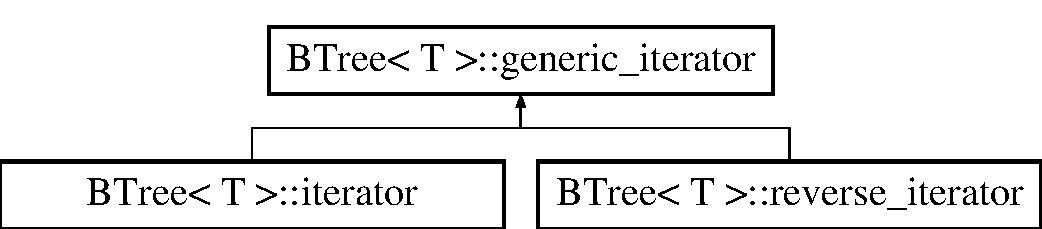
\includegraphics[height=2.000000cm]{classBTree_1_1generic__iterator}
\end{center}
\end{figure}
\subsection*{Public Member Functions}
\begin{DoxyCompactItemize}
\item 
\hypertarget{classBTree_1_1generic__iterator_a517efc73aa11d56062e0e02ca7a1df0d}{
{\bfseries generic\_\-iterator} (\hyperlink{classBTree}{BTree}$<$ T, Cmp $>$ $\ast$a, bool ended=false)}
\label{classBTree_1_1generic__iterator_a517efc73aa11d56062e0e02ca7a1df0d}

\item 
\hypertarget{classBTree_1_1generic__iterator_a0bbdec83e3269bc1c1b0c8f5f2fc94e0}{
const T \& {\bfseries operator$\ast$} () const }
\label{classBTree_1_1generic__iterator_a0bbdec83e3269bc1c1b0c8f5f2fc94e0}

\item 
\hypertarget{classBTree_1_1generic__iterator_abfb7311d27602e1dc909d9239457d272}{
bool {\bfseries operator!=} (const \hyperlink{classBTree}{BTree}$<$ T, Cmp $>$::\hyperlink{classBTree_1_1generic__iterator}{generic\_\-iterator} \&itCmp) const }
\label{classBTree_1_1generic__iterator_abfb7311d27602e1dc909d9239457d272}

\item 
\hypertarget{classBTree_1_1generic__iterator_ad8bfbbd09a1d55c8f2d6dda5d59a53e3}{
void {\bfseries operator++} (int ba)}
\label{classBTree_1_1generic__iterator_ad8bfbbd09a1d55c8f2d6dda5d59a53e3}

\item 
\hypertarget{classBTree_1_1generic__iterator_a66cbfb790427225fa52d1509c366e186}{
void {\bfseries operator-\/-\/} (int ba)}
\label{classBTree_1_1generic__iterator_a66cbfb790427225fa52d1509c366e186}

\item 
\hypertarget{classBTree_1_1generic__iterator_ae599b70c16505b2ff300c599dc7787a7}{
bool {\bfseries operator$<$} (const \hyperlink{classBTree}{BTree}$<$ T, Cmp $>$::\hyperlink{classBTree_1_1generic__iterator}{generic\_\-iterator} \&itCmp)}
\label{classBTree_1_1generic__iterator_ae599b70c16505b2ff300c599dc7787a7}

\item 
\hypertarget{classBTree_1_1generic__iterator_acf330d4cb3bc8fde3976571eaa3b5fb3}{
virtual void {\bfseries next} ()=0}
\label{classBTree_1_1generic__iterator_acf330d4cb3bc8fde3976571eaa3b5fb3}

\item 
\hypertarget{classBTree_1_1generic__iterator_aec59d969337997036619fba7fdf4da36}{
virtual void {\bfseries previous} ()=0}
\label{classBTree_1_1generic__iterator_aec59d969337997036619fba7fdf4da36}

\item 
\hypertarget{classBTree_1_1generic__iterator_ae1c991373b31b55adc78ec7102ed9c90}{
virtual void {\bfseries toFirstElement} ()=0}
\label{classBTree_1_1generic__iterator_ae1c991373b31b55adc78ec7102ed9c90}

\item 
\hypertarget{classBTree_1_1generic__iterator_a4609b12d5eb6066ebb0ef190bc289c81}{
\hyperlink{classBTree}{BTree}$<$ T, Cmp $>$::\hyperlink{classBTree_1_1generic__iterator}{generic\_\-iterator} {\bfseries operator+} (int inc) const }
\label{classBTree_1_1generic__iterator_a4609b12d5eb6066ebb0ef190bc289c81}

\item 
\hypertarget{classBTree_1_1generic__iterator_a92fb0c845dfeb8215d985b517e705947}{
void {\bfseries toParentR} ()}
\label{classBTree_1_1generic__iterator_a92fb0c845dfeb8215d985b517e705947}

\item 
\hypertarget{classBTree_1_1generic__iterator_acd2d74ca5d26a768e4ac92f8f02e7ca9}{
void {\bfseries toParentL} ()}
\label{classBTree_1_1generic__iterator_acd2d74ca5d26a768e4ac92f8f02e7ca9}

\end{DoxyCompactItemize}
\subsection*{Protected Member Functions}
\begin{DoxyCompactItemize}
\item 
\hypertarget{classBTree_1_1generic__iterator_aea0f779e6ae033a0b7a18ead33e5aeff}{
void {\bfseries toLeft} ()}
\label{classBTree_1_1generic__iterator_aea0f779e6ae033a0b7a18ead33e5aeff}

\item 
\hypertarget{classBTree_1_1generic__iterator_af3a3333fcf42f653efa5467a67387b79}{
void {\bfseries toRight} ()}
\label{classBTree_1_1generic__iterator_af3a3333fcf42f653efa5467a67387b79}

\item 
\hypertarget{classBTree_1_1generic__iterator_a511c737c31dda772fef150ad08216170}{
void {\bfseries toRightIndex} ()}
\label{classBTree_1_1generic__iterator_a511c737c31dda772fef150ad08216170}

\item 
\hypertarget{classBTree_1_1generic__iterator_a2357a1bf57af64373d98b1ad42e5fb3a}{
void {\bfseries toLeftIndex} ()}
\label{classBTree_1_1generic__iterator_a2357a1bf57af64373d98b1ad42e5fb3a}

\item 
\hypertarget{classBTree_1_1generic__iterator_a49aef3d72dbb1fe06c35da037b499082}{
bool {\bfseries ended} () const }
\label{classBTree_1_1generic__iterator_a49aef3d72dbb1fe06c35da037b499082}

\end{DoxyCompactItemize}
\subsection*{Protected Attributes}
\begin{DoxyCompactItemize}
\item 
\hypertarget{classBTree_1_1generic__iterator_ad64762fec58ac00d5ae5bbc672ed3a8a}{
\hyperlink{classBTree}{BTree}$<$ T, Cmp $>$ $\ast$ {\bfseries \_\-a}}
\label{classBTree_1_1generic__iterator_ad64762fec58ac00d5ae5bbc672ed3a8a}

\item 
\hypertarget{classBTree_1_1generic__iterator_a1f7da8be7535fa4a1ec4660344667053}{
\hyperlink{classNode}{Node}$<$ T, Cmp $>$ $\ast$ {\bfseries \_\-current\_\-node}}
\label{classBTree_1_1generic__iterator_a1f7da8be7535fa4a1ec4660344667053}

\item 
\hypertarget{classBTree_1_1generic__iterator_a198038019db667a9701f2f743158fbd3}{
int {\bfseries \_\-current\_\-index}}
\label{classBTree_1_1generic__iterator_a198038019db667a9701f2f743158fbd3}

\item 
\hypertarget{classBTree_1_1generic__iterator_a27a84badd0cbebab7e8eb85322e044cd}{
bool {\bfseries \_\-ended}}
\label{classBTree_1_1generic__iterator_a27a84badd0cbebab7e8eb85322e044cd}

\end{DoxyCompactItemize}
\subsubsection*{template$<$typename T, class Cmp = std::less$<$T$>$$>$ class BTree$<$ T, Cmp $>$::generic\_\-iterator}



The documentation for this class was generated from the following file:\begin{DoxyCompactItemize}
\item 
/media/Programmes/Dropbox/Univ nantes -\/ Master 1 ALMA/ProgGenerative/projet\_\-tp/Arbre\_\-b/src/BTree\_\-generic\_\-iterator.h\end{DoxyCompactItemize}

\hypertarget{classBTree_1_1iterator}{
\section{BTree$<$ T, Cmp $>$::iterator Class Reference}
\label{classBTree_1_1iterator}\index{BTree::iterator@{BTree::iterator}}
}
Inheritance diagram for BTree$<$ T, Cmp $>$::iterator:\begin{figure}[H]
\begin{center}
\leavevmode
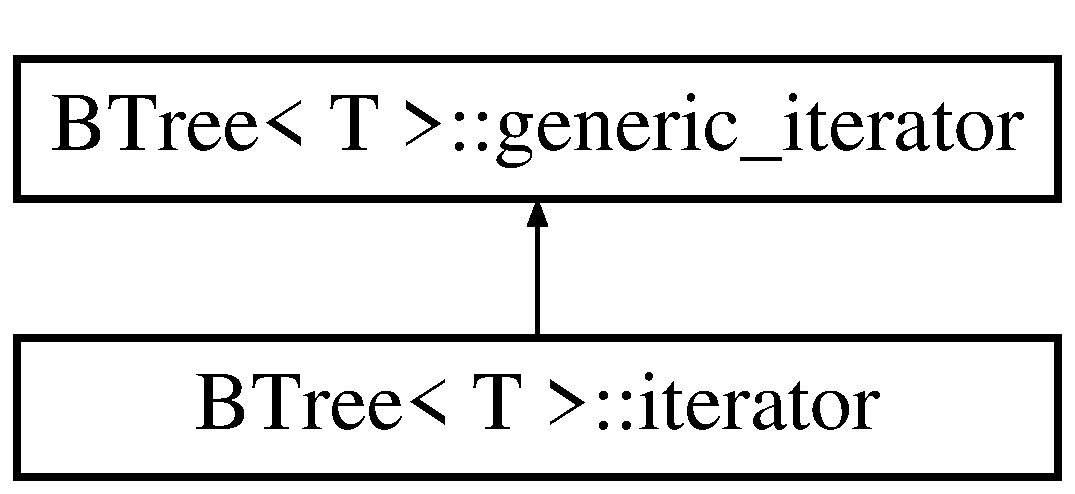
\includegraphics[height=2.000000cm]{classBTree_1_1iterator}
\end{center}
\end{figure}
\subsection*{Public Member Functions}
\begin{DoxyCompactItemize}
\item 
\hypertarget{classBTree_1_1iterator_ad34e487a9baf267daabe0dda42315553}{
{\bfseries iterator} (\hyperlink{classBTree}{BTree}$<$ T, Cmp $>$ $\ast$a, bool ended=false)}
\label{classBTree_1_1iterator_ad34e487a9baf267daabe0dda42315553}

\item 
\hypertarget{classBTree_1_1iterator_a539a8aec03bc81a5bbaf975ba56e5244}{
virtual void {\bfseries previous} ()}
\label{classBTree_1_1iterator_a539a8aec03bc81a5bbaf975ba56e5244}

\item 
\hypertarget{classBTree_1_1iterator_a993861d40f5da583f3c5af5db925c194}{
virtual void {\bfseries next} ()}
\label{classBTree_1_1iterator_a993861d40f5da583f3c5af5db925c194}

\item 
\hypertarget{classBTree_1_1iterator_a01fd8287c1734bdf5f16bdf03a593587}{
virtual void {\bfseries toFirstElement} ()}
\label{classBTree_1_1iterator_a01fd8287c1734bdf5f16bdf03a593587}

\end{DoxyCompactItemize}
\subsubsection*{template$<$typename T, class Cmp = std::less$<$T$>$$>$ class BTree$<$ T, Cmp $>$::iterator}



The documentation for this class was generated from the following file:\begin{DoxyCompactItemize}
\item 
/media/Programmes/Dropbox/Univ nantes -\/ Master 1 ALMA/ProgGenerative/projet\_\-tp/Arbre\_\-b/src/BTree\_\-iterator.h\end{DoxyCompactItemize}

\hypertarget{classNode}{
\section{Node$<$ T, Cmp $>$ Class Template Reference}
\label{classNode}\index{Node@{Node}}
}


\hyperlink{classBTree}{BTree} \hyperlink{classNode}{Node}. Contains Elements/Keys.  


\subsection*{Public Member Functions}
\begin{DoxyCompactItemize}
\item 
\hypertarget{classNode_ae2154f7c64506d0d7656aaa7bb728403}{
\hyperlink{classNode_ae2154f7c64506d0d7656aaa7bb728403}{Node} ()}
\label{classNode_ae2154f7c64506d0d7656aaa7bb728403}

\begin{DoxyCompactList}\small\item\em Make an new empty \hyperlink{classNode}{Node}. \item\end{DoxyCompactList}\item 
int \hyperlink{classNode_a00faa075c69d0e2015f7250d4e9c67c4}{addElement} (T element)
\begin{DoxyCompactList}\small\item\em Add an element to the \hyperlink{classNode}{Node} (not safe) \item\end{DoxyCompactList}\item 
int \hyperlink{classNode_aefc64b63487b63594388d386e5514ed0}{delElement} (const T \&element)
\begin{DoxyCompactList}\small\item\em Remove an element from the \hyperlink{classNode}{Node} (not safe) \item\end{DoxyCompactList}\item 
int \hyperlink{classNode_aebfe08afe47dc5a203d29c397378917c}{linkSon} (\hyperlink{classNode}{Node}$<$ T, Cmp $>$ $\ast$node)
\begin{DoxyCompactList}\small\item\em Add a \hyperlink{classNode}{Node} as son. \item\end{DoxyCompactList}\item 
void \hyperlink{classNode_a18a9441d84db7fc437c6105fcbeb7377}{unlinkSon} (\hyperlink{classNode}{Node}$<$ T, Cmp $>$ $\ast$node)
\begin{DoxyCompactList}\small\item\em Unlink a son \hyperlink{classNode}{Node} from this one. \item\end{DoxyCompactList}\item 
std::vector$<$ \hyperlink{classNode}{Node}$<$ T, Cmp $>$ $\ast$ $>$ \& \hyperlink{classNode_abe2b4ea866dac2c097420f41d0dc5b71}{getSons} ()
\begin{DoxyCompactList}\small\item\em Get a list of sons Nodes. \item\end{DoxyCompactList}\item 
std::vector$<$ T $>$ \& \hyperlink{classNode_ac9c04e56245dd777bfe3f677ac185beb}{getElements} ()
\begin{DoxyCompactList}\small\item\em Get a list of elements. \item\end{DoxyCompactList}\item 
\hyperlink{classNode}{Node}$<$ T, Cmp $>$ $\ast$ \hyperlink{classNode_a553d92ca84d985c43b12441cc45f923f}{getParent} ()
\begin{DoxyCompactList}\small\item\em Get parent node. \item\end{DoxyCompactList}\item 
\hyperlink{classNode}{Node}$<$ T, Cmp $>$ $\ast$ \hyperlink{classNode_acf4013394930061e49269798379096a5}{leftmostLeaf} ()
\begin{DoxyCompactList}\small\item\em Get the leftmost leaf from this node. \item\end{DoxyCompactList}\item 
\hyperlink{classNode}{Node}$<$ T, Cmp $>$ $\ast$ \hyperlink{classNode_ae690ca45669e86b221d98a6c26b3eee4}{rightmostLeaf} ()
\begin{DoxyCompactList}\small\item\em Get the rightmost leaf from this node. \item\end{DoxyCompactList}\item 
int \hyperlink{classNode_a7c7b4c56f7674dd028270a1bb8f880c6}{getElementPosition} (const T \&element) const 
\begin{DoxyCompactList}\small\item\em Get an element position in the element list. \item\end{DoxyCompactList}\item 
int \hyperlink{classNode_accd225fa793ba391ae96f2d77306bf49}{getSonPosition} (const \hyperlink{classNode}{Node}$<$ T, Cmp $>$ $\ast$son)
\begin{DoxyCompactList}\small\item\em Get an son node position in the son node list. \item\end{DoxyCompactList}\item 
bool \hyperlink{classNode_af734f4709cebbb317cd213ef0678149d}{isOverflowing} (int max\_\-size) const 
\begin{DoxyCompactList}\small\item\em Detect if node size exceeds the limit. \item\end{DoxyCompactList}\item 
bool \hyperlink{classNode_ac34f1b0085e87487b771848d059f9e28}{isUnderflowing} (int min\_\-size) const 
\begin{DoxyCompactList}\small\item\em Detect if node size deceeds the limit. \item\end{DoxyCompactList}\item 
bool \hyperlink{classNode_abcea6531f0a58ee2efeef2aa19dcd406}{contains} (const T \&element) const 
\begin{DoxyCompactList}\small\item\em Search for an element. \item\end{DoxyCompactList}\item 
bool \hyperlink{classNode_a0b4b829c1d9dd6818e9ec4e6d0b4d8c9}{isLeaf} () const 
\begin{DoxyCompactList}\small\item\em Detect if node is a leaf. \item\end{DoxyCompactList}\item 
\hypertarget{classNode_a78d6feccbe20a22af148b69c60bdec9e}{
void {\bfseries draw} (std::ostream \&flux)}
\label{classNode_a78d6feccbe20a22af148b69c60bdec9e}

\item 
int \hyperlink{classNode_ac87f195ec96daa6d1a52767467c4c9fb}{size} () const 
\begin{DoxyCompactList}\small\item\em Get number of elements in the \hyperlink{classNode}{Node}. \item\end{DoxyCompactList}\end{DoxyCompactItemize}


\subsection{Detailed Description}
\subsubsection*{template$<$typename T, class Cmp = std::less$<$T$>$$>$ class Node$<$ T, Cmp $>$}

\hyperlink{classBTree}{BTree} \hyperlink{classNode}{Node}. Contains Elements/Keys. \begin{DoxyAuthor}{Author}
Maxime OUAIRY 
\end{DoxyAuthor}


\subsection{Member Function Documentation}
\hypertarget{classNode_a00faa075c69d0e2015f7250d4e9c67c4}{
\index{Node@{Node}!addElement@{addElement}}
\index{addElement@{addElement}!Node@{Node}}
\subsubsection[{addElement}]{\setlength{\rightskip}{0pt plus 5cm}template$<$typename T, class Cmp = std::less$<$T$>$$>$ int {\bf Node}$<$ T, Cmp $>$::addElement (
\begin{DoxyParamCaption}
\item[{T}]{element}
\end{DoxyParamCaption}
)}}
\label{classNode_a00faa075c69d0e2015f7250d4e9c67c4}


Add an element to the \hyperlink{classNode}{Node} (not safe) 


\begin{DoxyParams}{Parameters}
{\em element} & Element to insert in the \hyperlink{classNode}{Node} \\
\hline
\end{DoxyParams}
\begin{DoxyReturn}{Returns}
Index of inserted element 
\end{DoxyReturn}
\hypertarget{classNode_abcea6531f0a58ee2efeef2aa19dcd406}{
\index{Node@{Node}!contains@{contains}}
\index{contains@{contains}!Node@{Node}}
\subsubsection[{contains}]{\setlength{\rightskip}{0pt plus 5cm}template$<$typename T, class Cmp = std::less$<$T$>$$>$ bool {\bf Node}$<$ T, Cmp $>$::contains (
\begin{DoxyParamCaption}
\item[{const T \&}]{element}
\end{DoxyParamCaption}
) const}}
\label{classNode_abcea6531f0a58ee2efeef2aa19dcd406}


Search for an element. 


\begin{DoxyParams}{Parameters}
{\em element} & Reference to searched element \\
\hline
\end{DoxyParams}
\begin{DoxyReturn}{Returns}
true if element is in this node, false otherwise 
\end{DoxyReturn}
\hypertarget{classNode_aefc64b63487b63594388d386e5514ed0}{
\index{Node@{Node}!delElement@{delElement}}
\index{delElement@{delElement}!Node@{Node}}
\subsubsection[{delElement}]{\setlength{\rightskip}{0pt plus 5cm}template$<$typename T, class Cmp = std::less$<$T$>$$>$ int {\bf Node}$<$ T, Cmp $>$::delElement (
\begin{DoxyParamCaption}
\item[{const T \&}]{element}
\end{DoxyParamCaption}
)}}
\label{classNode_aefc64b63487b63594388d386e5514ed0}


Remove an element from the \hyperlink{classNode}{Node} (not safe) 


\begin{DoxyParams}{Parameters}
{\em element} & Element to delete from the \hyperlink{classNode}{Node} \\
\hline
\end{DoxyParams}
\begin{DoxyReturn}{Returns}
Old index of deleted element, if found. -\/1 otherwise 
\end{DoxyReturn}
\hypertarget{classNode_a7c7b4c56f7674dd028270a1bb8f880c6}{
\index{Node@{Node}!getElementPosition@{getElementPosition}}
\index{getElementPosition@{getElementPosition}!Node@{Node}}
\subsubsection[{getElementPosition}]{\setlength{\rightskip}{0pt plus 5cm}template$<$typename T, class Cmp = std::less$<$T$>$$>$ int {\bf Node}$<$ T, Cmp $>$::getElementPosition (
\begin{DoxyParamCaption}
\item[{const T \&}]{element}
\end{DoxyParamCaption}
) const}}
\label{classNode_a7c7b4c56f7674dd028270a1bb8f880c6}


Get an element position in the element list. 


\begin{DoxyParams}{Parameters}
{\em element} & Reference to the element to locate \\
\hline
\end{DoxyParams}
\begin{DoxyReturn}{Returns}
Index of element in list. -\/1 otherwise 
\end{DoxyReturn}
\hypertarget{classNode_ac9c04e56245dd777bfe3f677ac185beb}{
\index{Node@{Node}!getElements@{getElements}}
\index{getElements@{getElements}!Node@{Node}}
\subsubsection[{getElements}]{\setlength{\rightskip}{0pt plus 5cm}template$<$typename T, class Cmp = std::less$<$T$>$$>$ std::vector$<$T$>$\& {\bf Node}$<$ T, Cmp $>$::getElements (
\begin{DoxyParamCaption}
{}
\end{DoxyParamCaption}
)}}
\label{classNode_ac9c04e56245dd777bfe3f677ac185beb}


Get a list of elements. 

\begin{DoxyReturn}{Returns}
A vector reference of elements list 
\end{DoxyReturn}
\hypertarget{classNode_a553d92ca84d985c43b12441cc45f923f}{
\index{Node@{Node}!getParent@{getParent}}
\index{getParent@{getParent}!Node@{Node}}
\subsubsection[{getParent}]{\setlength{\rightskip}{0pt plus 5cm}template$<$typename T, class Cmp = std::less$<$T$>$$>$ {\bf Node}$<$T,Cmp$>$$\ast$ {\bf Node}$<$ T, Cmp $>$::getParent (
\begin{DoxyParamCaption}
{}
\end{DoxyParamCaption}
)}}
\label{classNode_a553d92ca84d985c43b12441cc45f923f}


Get parent node. 

\begin{DoxyReturn}{Returns}
A pointer to parent \hyperlink{classNode}{Node}. NULL if Root. 
\end{DoxyReturn}
\hypertarget{classNode_accd225fa793ba391ae96f2d77306bf49}{
\index{Node@{Node}!getSonPosition@{getSonPosition}}
\index{getSonPosition@{getSonPosition}!Node@{Node}}
\subsubsection[{getSonPosition}]{\setlength{\rightskip}{0pt plus 5cm}template$<$typename T, class Cmp = std::less$<$T$>$$>$ int {\bf Node}$<$ T, Cmp $>$::getSonPosition (
\begin{DoxyParamCaption}
\item[{const {\bf Node}$<$ T, Cmp $>$ $\ast$}]{son}
\end{DoxyParamCaption}
)}}
\label{classNode_accd225fa793ba391ae96f2d77306bf49}


Get an son node position in the son node list. 


\begin{DoxyParams}{Parameters}
{\em son} & Reference to the element to son node \\
\hline
\end{DoxyParams}
\begin{DoxyReturn}{Returns}
Index of son node in list. -\/1 otherwise 
\end{DoxyReturn}
\hypertarget{classNode_abe2b4ea866dac2c097420f41d0dc5b71}{
\index{Node@{Node}!getSons@{getSons}}
\index{getSons@{getSons}!Node@{Node}}
\subsubsection[{getSons}]{\setlength{\rightskip}{0pt plus 5cm}template$<$typename T, class Cmp = std::less$<$T$>$$>$ std::vector$<$ {\bf Node}$<$T,Cmp$>$$\ast$ $>$\& {\bf Node}$<$ T, Cmp $>$::getSons (
\begin{DoxyParamCaption}
{}
\end{DoxyParamCaption}
)}}
\label{classNode_abe2b4ea866dac2c097420f41d0dc5b71}


Get a list of sons Nodes. 

\begin{DoxyReturn}{Returns}
A vector reference of sons list 
\end{DoxyReturn}
\hypertarget{classNode_a0b4b829c1d9dd6818e9ec4e6d0b4d8c9}{
\index{Node@{Node}!isLeaf@{isLeaf}}
\index{isLeaf@{isLeaf}!Node@{Node}}
\subsubsection[{isLeaf}]{\setlength{\rightskip}{0pt plus 5cm}template$<$typename T, class Cmp = std::less$<$T$>$$>$ bool {\bf Node}$<$ T, Cmp $>$::isLeaf (
\begin{DoxyParamCaption}
{}
\end{DoxyParamCaption}
) const}}
\label{classNode_a0b4b829c1d9dd6818e9ec4e6d0b4d8c9}


Detect if node is a leaf. 


\begin{DoxyParams}{Parameters}
{\em element} & Reference to searched element \\
\hline
\end{DoxyParams}
\begin{DoxyReturn}{Returns}
true if element is in this node, false otherwise 
\end{DoxyReturn}
\hypertarget{classNode_af734f4709cebbb317cd213ef0678149d}{
\index{Node@{Node}!isOverflowing@{isOverflowing}}
\index{isOverflowing@{isOverflowing}!Node@{Node}}
\subsubsection[{isOverflowing}]{\setlength{\rightskip}{0pt plus 5cm}template$<$typename T, class Cmp = std::less$<$T$>$$>$ bool {\bf Node}$<$ T, Cmp $>$::isOverflowing (
\begin{DoxyParamCaption}
\item[{int}]{max\_\-size}
\end{DoxyParamCaption}
) const}}
\label{classNode_af734f4709cebbb317cd213ef0678149d}


Detect if node size exceeds the limit. 


\begin{DoxyParams}{Parameters}
{\em max\_\-size} & Maximum node size \\
\hline
\end{DoxyParams}
\begin{DoxyReturn}{Returns}
true if node size exceeds max\_\-size. false otherwise 
\end{DoxyReturn}
\hypertarget{classNode_ac34f1b0085e87487b771848d059f9e28}{
\index{Node@{Node}!isUnderflowing@{isUnderflowing}}
\index{isUnderflowing@{isUnderflowing}!Node@{Node}}
\subsubsection[{isUnderflowing}]{\setlength{\rightskip}{0pt plus 5cm}template$<$typename T, class Cmp = std::less$<$T$>$$>$ bool {\bf Node}$<$ T, Cmp $>$::isUnderflowing (
\begin{DoxyParamCaption}
\item[{int}]{min\_\-size}
\end{DoxyParamCaption}
) const}}
\label{classNode_ac34f1b0085e87487b771848d059f9e28}


Detect if node size deceeds the limit. 


\begin{DoxyParams}{Parameters}
{\em min\_\-size} & Minimum node size \\
\hline
\end{DoxyParams}
\begin{DoxyReturn}{Returns}
true if node size deceeds max\_\-size. false otherwise 
\end{DoxyReturn}
\hypertarget{classNode_acf4013394930061e49269798379096a5}{
\index{Node@{Node}!leftmostLeaf@{leftmostLeaf}}
\index{leftmostLeaf@{leftmostLeaf}!Node@{Node}}
\subsubsection[{leftmostLeaf}]{\setlength{\rightskip}{0pt plus 5cm}template$<$typename T, class Cmp = std::less$<$T$>$$>$ {\bf Node}$<$T,Cmp$>$$\ast$ {\bf Node}$<$ T, Cmp $>$::leftmostLeaf (
\begin{DoxyParamCaption}
{}
\end{DoxyParamCaption}
)}}
\label{classNode_acf4013394930061e49269798379096a5}


Get the leftmost leaf from this node. 

\begin{DoxyReturn}{Returns}
A pointer to leftmost leaf node 
\end{DoxyReturn}
\hypertarget{classNode_aebfe08afe47dc5a203d29c397378917c}{
\index{Node@{Node}!linkSon@{linkSon}}
\index{linkSon@{linkSon}!Node@{Node}}
\subsubsection[{linkSon}]{\setlength{\rightskip}{0pt plus 5cm}template$<$typename T, class Cmp = std::less$<$T$>$$>$ int {\bf Node}$<$ T, Cmp $>$::linkSon (
\begin{DoxyParamCaption}
\item[{{\bf Node}$<$ T, Cmp $>$ $\ast$}]{node}
\end{DoxyParamCaption}
)}}
\label{classNode_aebfe08afe47dc5a203d29c397378917c}


Add a \hyperlink{classNode}{Node} as son. 


\begin{DoxyParams}{Parameters}
{\em node} & Future son \hyperlink{classNode}{Node} \\
\hline
\end{DoxyParams}
\begin{DoxyReturn}{Returns}
Index of inserted son 
\end{DoxyReturn}
\hypertarget{classNode_ae690ca45669e86b221d98a6c26b3eee4}{
\index{Node@{Node}!rightmostLeaf@{rightmostLeaf}}
\index{rightmostLeaf@{rightmostLeaf}!Node@{Node}}
\subsubsection[{rightmostLeaf}]{\setlength{\rightskip}{0pt plus 5cm}template$<$typename T, class Cmp = std::less$<$T$>$$>$ {\bf Node}$<$T,Cmp$>$$\ast$ {\bf Node}$<$ T, Cmp $>$::rightmostLeaf (
\begin{DoxyParamCaption}
{}
\end{DoxyParamCaption}
)}}
\label{classNode_ae690ca45669e86b221d98a6c26b3eee4}


Get the rightmost leaf from this node. 

\begin{DoxyReturn}{Returns}
A pointer to rightmost leaf node 
\end{DoxyReturn}
\hypertarget{classNode_ac87f195ec96daa6d1a52767467c4c9fb}{
\index{Node@{Node}!size@{size}}
\index{size@{size}!Node@{Node}}
\subsubsection[{size}]{\setlength{\rightskip}{0pt plus 5cm}template$<$typename T, class Cmp = std::less$<$T$>$$>$ int {\bf Node}$<$ T, Cmp $>$::size (
\begin{DoxyParamCaption}
{}
\end{DoxyParamCaption}
) const}}
\label{classNode_ac87f195ec96daa6d1a52767467c4c9fb}


Get number of elements in the \hyperlink{classNode}{Node}. 

\begin{DoxyReturn}{Returns}
Current number of elements inserted 
\end{DoxyReturn}
\hypertarget{classNode_a18a9441d84db7fc437c6105fcbeb7377}{
\index{Node@{Node}!unlinkSon@{unlinkSon}}
\index{unlinkSon@{unlinkSon}!Node@{Node}}
\subsubsection[{unlinkSon}]{\setlength{\rightskip}{0pt plus 5cm}template$<$typename T, class Cmp = std::less$<$T$>$$>$ void {\bf Node}$<$ T, Cmp $>$::unlinkSon (
\begin{DoxyParamCaption}
\item[{{\bf Node}$<$ T, Cmp $>$ $\ast$}]{node}
\end{DoxyParamCaption}
)}}
\label{classNode_a18a9441d84db7fc437c6105fcbeb7377}


Unlink a son \hyperlink{classNode}{Node} from this one. 


\begin{DoxyParams}{Parameters}
{\em node} & Son \hyperlink{classNode}{Node} to unlink \\
\hline
\end{DoxyParams}


The documentation for this class was generated from the following file:\begin{DoxyCompactItemize}
\item 
/media/Programmes/Dropbox/Univ nantes -\/ Master 1 ALMA/ProgGenerative/projet\_\-tp/Arbre\_\-b/src/Node.h\end{DoxyCompactItemize}

\hypertarget{classBTree_1_1reverse__iterator}{
\section{BTree$<$ T $>$::reverse\_\-iterator Class Reference}
\label{classBTree_1_1reverse__iterator}\index{BTree::reverse\_\-iterator@{BTree::reverse\_\-iterator}}
}
Inheritance diagram for BTree$<$ T $>$::reverse\_\-iterator:\begin{figure}[H]
\begin{center}
\leavevmode
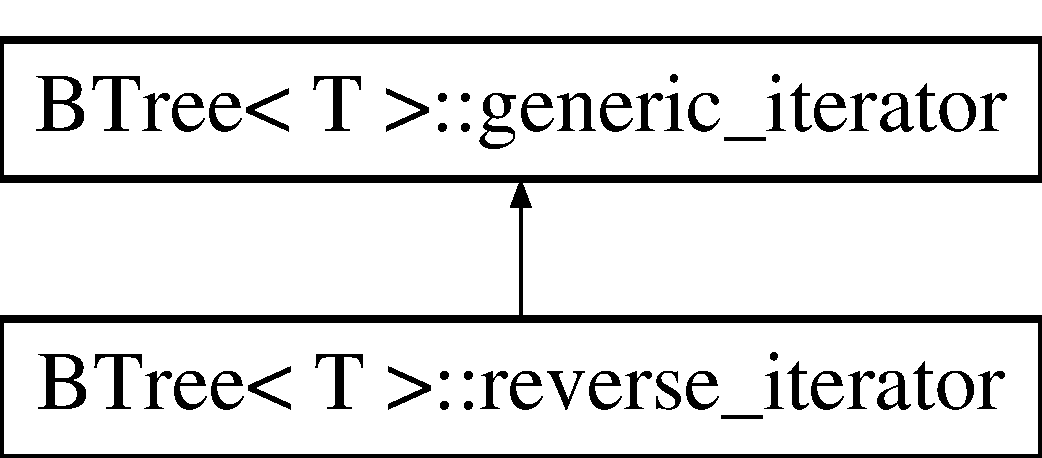
\includegraphics[height=2.000000cm]{classBTree_1_1reverse__iterator}
\end{center}
\end{figure}
\subsection*{Public Member Functions}
\begin{DoxyCompactItemize}
\item 
\hypertarget{classBTree_1_1reverse__iterator_a6fa59c7abfb1da84d37681c33e5d1794}{
{\bfseries reverse\_\-iterator} (\hyperlink{classBTree}{BTree}$<$ T $>$ $\ast$a, bool ended=false)}
\label{classBTree_1_1reverse__iterator_a6fa59c7abfb1da84d37681c33e5d1794}

\item 
\hypertarget{classBTree_1_1reverse__iterator_aba79def66924c5b31fb71f86a450368f}{
virtual void {\bfseries previous} ()}
\label{classBTree_1_1reverse__iterator_aba79def66924c5b31fb71f86a450368f}

\item 
\hypertarget{classBTree_1_1reverse__iterator_ae624f8b196dd4b6af8e8cb1b2911671b}{
virtual void {\bfseries next} ()}
\label{classBTree_1_1reverse__iterator_ae624f8b196dd4b6af8e8cb1b2911671b}

\item 
\hypertarget{classBTree_1_1reverse__iterator_a413004d00bf9f246407c267c907cb896}{
virtual void {\bfseries toFirstElement} ()}
\label{classBTree_1_1reverse__iterator_a413004d00bf9f246407c267c907cb896}

\end{DoxyCompactItemize}
\subsubsection*{template$<$typename T$>$ class BTree$<$ T $>$::reverse\_\-iterator}



The documentation for this class was generated from the following file:\begin{DoxyCompactItemize}
\item 
/media/Programmes/Dropbox/Univ nantes -\/ Master 1 ALMA/ProgGenerative/projet\_\-tp/Arbre\_\-b/src/BTree\_\-reverse\_\-iterator.h\end{DoxyCompactItemize}

\printindex
\end{document}
